\documentclass{article}
\usepackage[utf8]{inputenc}
\usepackage{hyperref}
\usepackage{amsmath,amssymb}
\usepackage{graphicx}
\usepackage{float}
\usepackage[margin=2.5cm]{geometry}

\newcommand{\mbf}[1]{\mathbf{#1}}
\newcommand{\be}{\begin{equation}}
\newcommand{\ee}{\end{equation}}
\newcommand{\mcl}[1]{\mathcal{#1}}

\title{Multifrequency Analysis: $50 \times 50$ Cell Model\vspace{-1em}}
\author{(notes)}
\date{}

\begin{document}
\maketitle

%% ==================================================================
\section{Frequency-Specific Overfitting in Single-Frequency Optimization}
%% ==================================================================

Neural network optimization of the cloak material parameters can easily achieve
excellent cloaking performance at a single design frequency.
However, optimizing at one frequency
produces a highly frequency-specific solution that fails to generalize
to other frequencies.

Figure~\ref{fig:freq_overfitting} illustrates this phenomenon by comparing
two optimization runs on identical $50 \times 50$ cell models, trained at
different frequencies (2.5\,kHz and 3.0\,kHz).
Each model is then evaluated across the range 1.0--4.0\,kHz.

\begin{figure}[H]
  \centering
  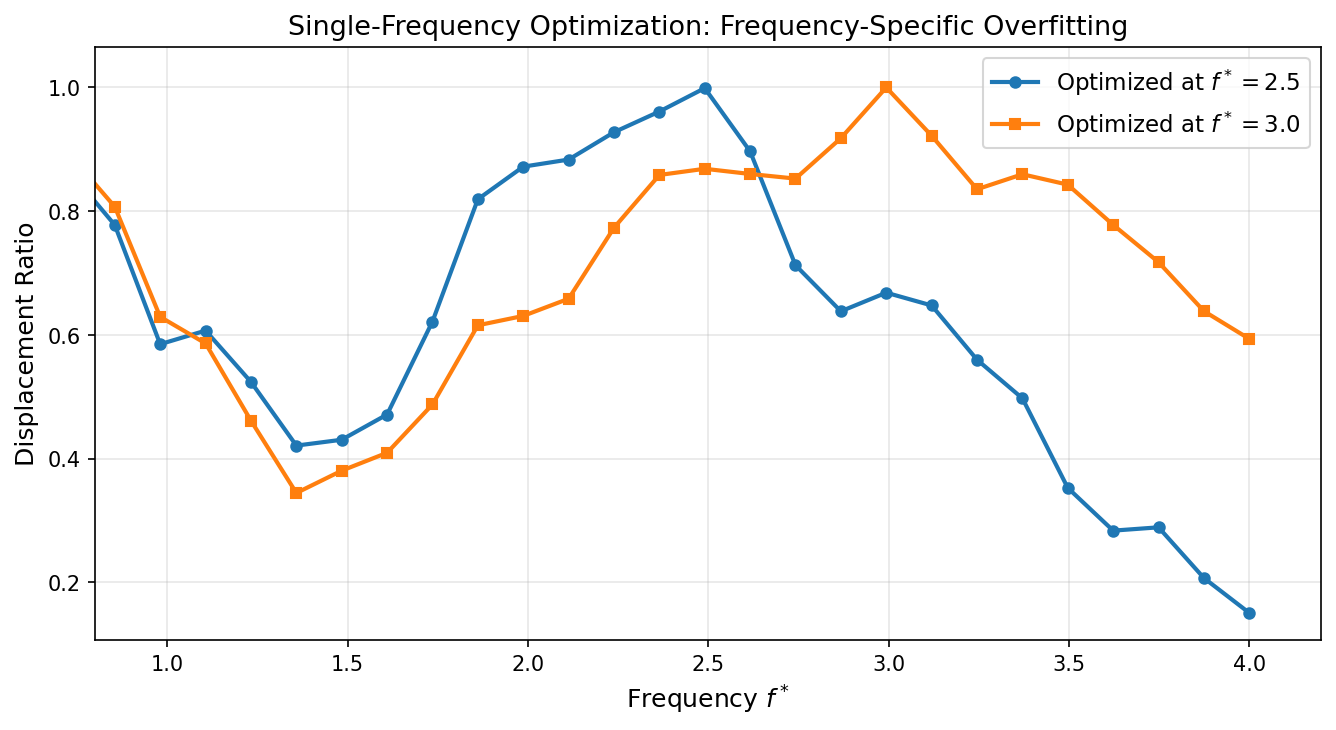
\includegraphics[width=0.9\linewidth]{single_freq_comparison.png}
  \caption{Frequency response of two independently optimized $50 \times 50$ cell models,
  each trained at a single frequency (2.5\,kHz and 3.0\,kHz).
  The sharp minima at the training frequencies illustrate frequency-specific
  overfitting; performance away from the design frequency degrades significantly.}
  \label{fig:freq_overfitting}
\end{figure}

%% ==================================================================
\section{Multifrequency Objective}
%% ==================================================================

To address narrow-band overfitting, we adopt a multifrequency training objective
that enforces broadband cloaking performance across a range of frequencies.
The loss function is modified to evaluate cloaking distortion at
multiple frequencies and sum their contributions, ensuring that the optimization
does not trade performance at one frequency for another. Figure~\ref{fig:multifreq_sweep} shows the cloaking performance of a single
$50 \times 50$ cell model optimized using the multifrequency objective.

\begin{figure}[H]
  \centering
  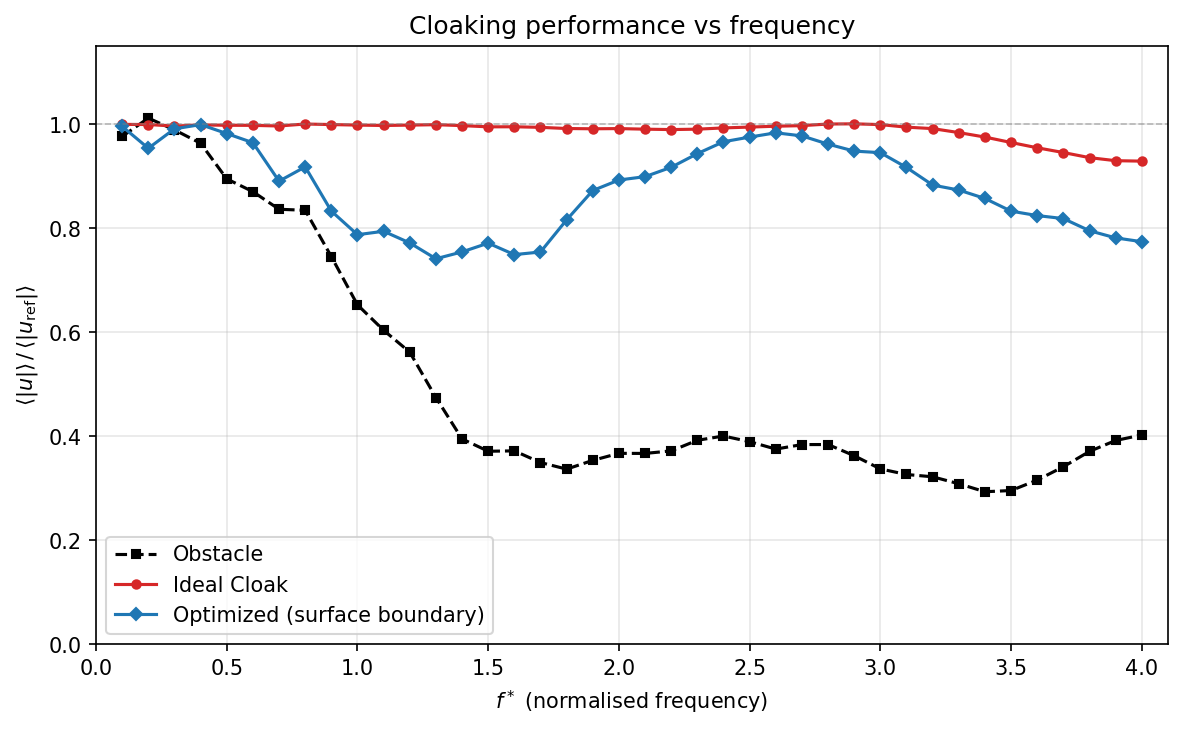
\includegraphics[width=0.8\linewidth]{multifreq_sweep.png}
  \caption{Frequency sweep of the multifrequency-optimized $50 \times 50$ cell model.}
  \label{fig:multifreq_sweep}
\end{figure}

%% ==================================================================
\section{Floquet--Bloch Analysis}
%% ==================================================================

The multifrequency-optimized material field is analyzed through Floquet--Bloch
band structure computation at the optimal parameters (Figure~\ref{fig:bloch}).

\begin{figure}[H]
  \centering
  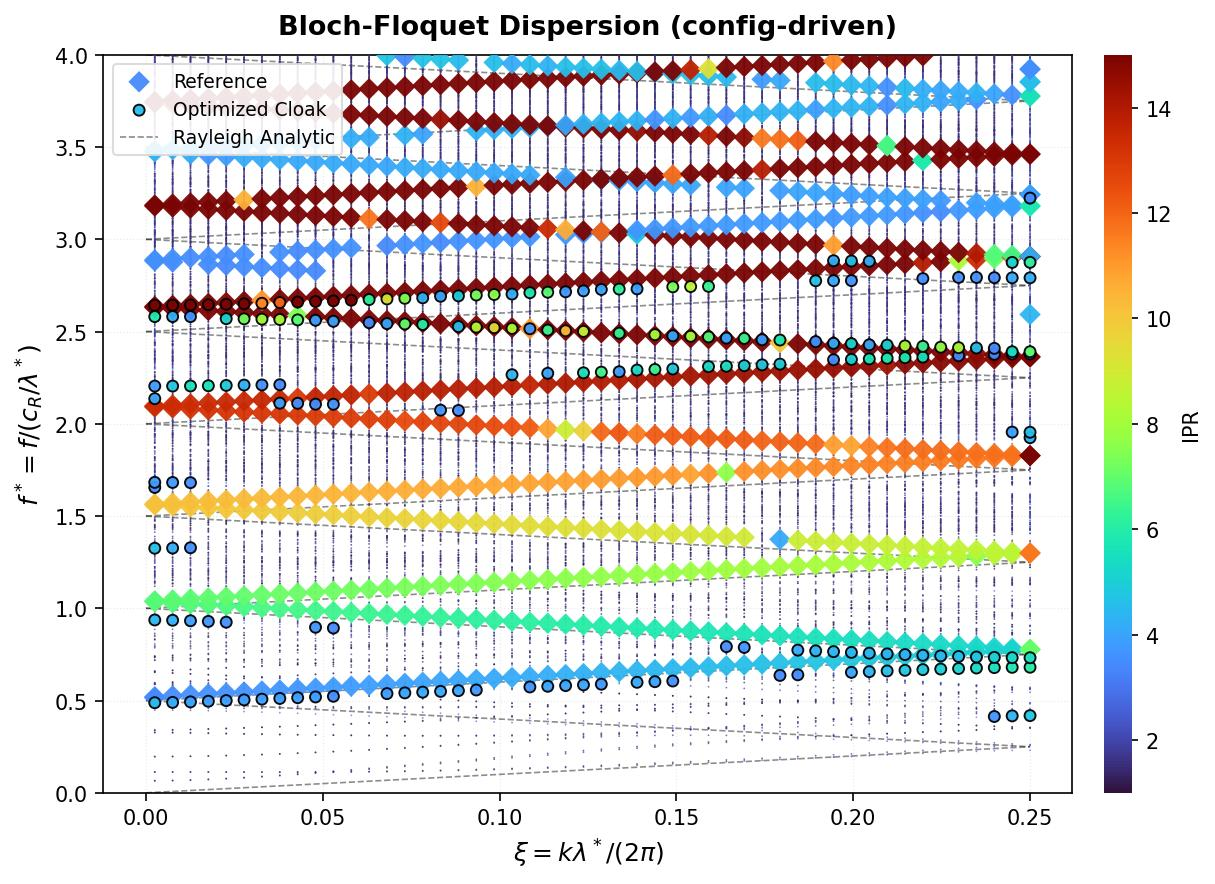
\includegraphics[width=0.85\linewidth]{bloch.jpg}
  \caption{Floquet--Bloch band structure analysis of the multifrequency-optimized
  $50 \times 50$ cell model.}
  \label{fig:bloch}
\end{figure}

\end{document}
